\section{実装}

\subsection{データセット}
学習データは CC-100 日本語版と字幕コーパス（OpenSubtitles 日本語，JESC）を
同程度の件数で交互に混合して構築する．
原文を「。！？」で文に分割し，空白を詰めたうえで，
日本語を含み長さ 2--40 字の文のみを残す．
各文を母音化し，母音列・文脈・正解文の 3 項組を生成する．
文脈には同一原文内の直前の文を入れるが，
既定で割合 0.5 で文脈なしに落とし，母音列のみでも候補生成できるよう学習する．
学習に用いたデータの実件数は train 660{,}007 件，eval 1{,}309 件であった．

\subsection{プロンプトと損失設計}
学習・推論・API で完全一致するプロンプトを用いる．
\begin{quote}\footnotesize
\texttt{あなたは日本語IMEの文復元器です。}\\
\texttt{母音列(a/i/u/e/o/n)から元の文を復元してください。}\\
\texttt{CTX: \{ctx\}}\\
\texttt{VOWELS: \{vowels\}}\\
\texttt{SENTENCE:}
\end{quote}
\texttt{SENTENCE:} 以降を生成対象とし，プロンプト部は損失計算から除外して
文＋EOS のみに損失を与える．

\subsection{モデルとハイパーパラメータ}
ベースモデルは MiniCPM4-0.5B（revision \texttt{2aaa97c53d} を pin）であり，
bfloat16 で読み込む．LoRA の対象は注意機構と MLP の全線形層
（\texttt{q/k/v/o\_proj}，\texttt{gate/up/down\_proj}）である．
主な設定値を表\ref{tab:setup}に示す．
実際に完了した学習は，
学習データ上限 2{,}000{,}000 件（実データ上限により 660{,}007 件），
epoch 2，バッチ 8，勾配累積 4（実効バッチ 32），最大系列長 128，
学習率 $1\times10^{-4}$，optimizer は AdamW であった．
学習は 41{,}250 ステップで完了している．
学習・評価損失はともに約 1.2 付近まで低下した（図\ref{fig:flow} 右）．
実験環境は GPU が NVIDIA GeForce RTX 5060 Ti，OS は Ubuntu 24.04.4 LTS，
PyTorch 2.12.0 である．

\begin{table}[t]
  \centering\small
  \caption{実験設定}
  \label{tab:setup}
  \begin{tabular}{ll}
    \toprule
    項目 & 値 \\
    \midrule
    base model & openbmb/MiniCPM4-0.5B \\
    training data & CC-100-ja + 字幕（混合）\\
    eval data & 同分布の hold-out \\
    train records & 660{,}007（上限 2{,}000{,}000 指定）\\
    eval records & 1{,}309 \\
    epoch & 2 \\
    batch size & 8 \\
    grad accum & 4（実効 32）\\
    max seq len & 128 \\
    LoRA rank $r$ & 32 \\
    LoRA alpha $\alpha$ & 64 \\
    LoRA dropout & 0.05 \\
    target modules & q,k,v,o,gate,up,down\_proj \\
    learning rate & $1\times10^{-4}$ \\
    optimizer & AdamW \\
    GPU & NVIDIA GeForce RTX 5060 Ti \\
    OS & Ubuntu 24.04.4 LTS \\
    PyTorch & 2.12.0 \\
    \bottomrule
  \end{tabular}
\end{table}

\begin{figure}[t]
  \centering
  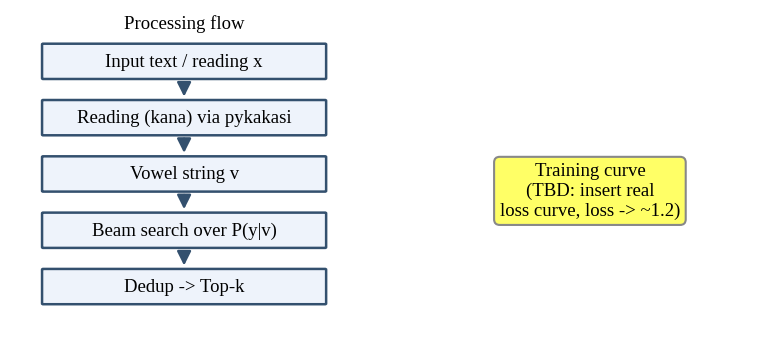
\includegraphics[width=0.95\columnwidth]{figures/fig_flow.png}
  \caption{母音入力から候補提示までの処理フロー（左）と学習曲線（右）．}
  \label{fig:flow}
\end{figure}

\subsection{推論・配信}
推論はビーム幅 8・最大新規トークン 64 で行い，重複除去した上位 $k$ 件を返す．
HTTP API も同一プロンプトで実装されている．

\subsection{母音キーボードの実装}
提案手法に基づき，スマートフォン上で動作する母音キーボードを試作した
（図\ref{fig:keyboard}）．キーは 5 母音（\texttt{a, i, u, e, o}）と撥音（\texttt{n}）
を中心とした最小限の構成であり，各キーを大きく配置している。
キー数を絞ったことで画面においてキーボードが占める割合は小さく，
表示領域を広く確保できる。

\begin{figure}[t]
  \centering
  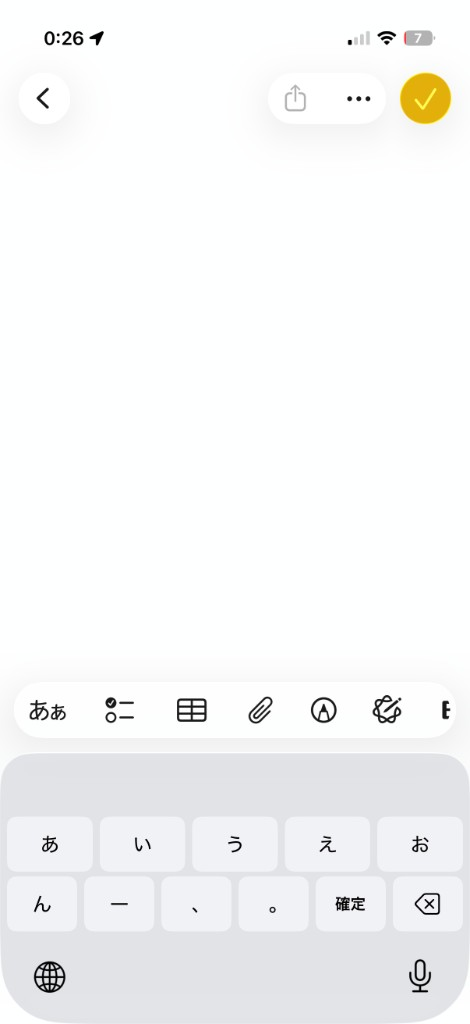
\includegraphics[height=0.42\textheight]{figures/fig_keyboard.png}
  \caption{試作した母音キーボードの画面例．5 母音と撥音を中心とした少数キー構成により，各キーを大きく配置している．}
  \label{fig:keyboard}
\end{figure}
